%%%%%%%%%%%%%%%%%%%%%%%%%%%%%%%%%%%%%%%%%%%%%%%%%%%%%%%%%%%%%%%%%%%%%%%%%%%%
%% Trim Size : 11in x 8.5in
%% Text Area : 9.in (include Runningheads) x 7in
%% ws-jai.tex, 26 April 2012
%% Tex file to use with ws-jai.cls written in Latex2E.
%% The content, structure, format and layout of this style file is the
%% property of World Scientific Publishing Co. Pte. Ltd.
%%%%%%%%%%%%%%%%%%%%%%%%%%%%%%%%%%%%%%%%%%%%%%%%%%%%%%%%%%%%%%%%%%%%%%%%%%%%
%%

%\documentclass[draft]{ws-jai}
\documentclass{ws-jai}
\usepackage[flushleft]{threeparttable}
%% \usepackage{caption}
%% \usepackage{subcaption}
\begin{document}

\catchline{}{}{}{}{} % Publisher's Area please ignore

\markboth{P.Prasad}{The AARTFAAC Radio Sky Monitor: System Design and Implementation}

\title{The AARTFAAC Radio Sky Monitor: System Design and Implementation}

\author{Peeyush Prasad$^\dagger$, Folkert Huizinga$^\S$, Eric Kooistra$^\ddagger$, Daniel van der Schuur $^\ddagger$, Andre Gunst $^\ddagger$, John Romein $^\ddagger$, Mark Kuiack $^\S$, Gijs Molenaar $^\S$ and Ralph Wijers$^\S$}

\address{
$^\dagger$Anton Pannekoek Institute, University of Amsterdam, Amsterdam, The Netherlands, p.prasad@uva.nl\\
$^\ddagger$ASTRON, Oude Hoogeveensedijk, 7991PD, The Netherlands\\
$^\S$Anton Pannekoek Institute, University of Amsterdam, Amsterdam\\
}

\maketitle

\corres{$^\dagger$Corresponding Author}

\begin{history}
\received{(to be inserted by publisher)};
\revised{(to be inserted by publisher)};
\accepted{(to be inserted by publisher)};
\end{history}

\begin{abstract}
The Amsterdam-ASTRON  Radio Transients  Facility And Analysis  Center (AARTFAAC)
array  is  a sensitive,  all-sky  radio  transient  detector  based on  the  Low
Frequency Array (LOFAR).  It generates images  of the low frequency radio sky in
near real-time  with spatial resolution of  10s of arcmin, MHz  bandwidths and a
time cadence of a few seconds. The image timeseries are then monitored for short
and bright radio  transients. On detection of a transient,  low latency triggers
will be  generated for LOFAR,  which can  carry out follow-up  observations.  In
this paper,  we describe  our heterogeneous, hierarchical  design to  manage the
~240 Gbps raw data rate, and the TODO TFLOPs of computing needed.  We discuss the
implementation  of   the  instrumentation,  its  capabilities,   and  show  some
commissioning results.
\end{abstract}

\keywords{Radio Interferometry, Imaging, Radio Transients, Correlators}

\section{\label{sec:Introduction}Introduction}

\noindent Transient astronomy  deals with the detection  and characterization of
celestial transients, sources in the  sky whose detectable properties can change
on short timescales.   These explosive events provide insight into  a variety of
astrophysics,  ranging from  emission mechanisms  of jets  to properties  of the
intervening  medium \citep{fender2006lofar,lazio2009dynamic}.  

%% Studies of short  duration radio emission from such objects  has been restricted
%% to   either    very   short   timescales   (milliseconds    to   seconds,   e.g.
%% Pulsars[TODO:Ref]),   or  to   comparatively   longer   timescales  (months   to
%% years[TODO:Ref])   primarily  due   to  observational   time,  or   instrumental
%% constraints,  the  former due  to  the  narrow  fields  of view  of  traditional
%% instruments.

For time resolved observations, radio  instrumentation is generally available in
two  classes; Firstly,  a  single  dish or  phased  array  beam formed  approach
characterized by  high time and frequency  resolution, wide fields of  view of a
few degrees but poor spatial resolution. This mode is optimized for detection of
coherent    sources,     which    are     expected    to    emit     on    short
timescales. Interferometric  aperture synthesis observations is  the other mode,
providing high spatial resolutions, but  poor time resolution, typically needing
several hours of observation time to build  up adequate coverage in the UV plane
via  earth rotation  aperture synthesis.   This  mode is  optimal for  detecting
incoherent  sources,  whose  timescales  of   emission  are  much  slower.

The serendipitous discovery of a new  class of radio transient termed Fast Radio
Bursts  (FRBs)\citep{spitler2015fast,   thornton2013population}  has  galvanized
interest in the field.  The detected  FRBs are characterized by large associated
dispersion   measures,  high   brightness  and   short  timescales.    They  are
non-repeating for  the most part. Their  unknown origin requires not  only their
discovery, but also  rapid followup over a large wavelength  regime to establish
emission  phenomena  and  associated  parameters.   A  recent  example  of  this
requirement is the detection by \citet{stewart2016lofar} of a ~20Jy transient in
60MHz  LOFAR  data,  whose  characterization  has  suffered  due  to  inadequate
multi-wavelength  coverage. As  a consequence,  large  field of  view radio  sky
monitors are being  developed to continuously survey large parts  of the visible
sky  with shallow  sensitivity and  at high  time resolution.  A trigger  can be
generated on the  reliable detection of a transient in  near real-time, allowing
other telescopes to carry out follow-up observations.

% \item Suitability of low frequency observations \\
% <TODO: Paragraph about  transient sources, some stuff about  spectral indices of
% coherent emission and  expected class of sources, at what  brightness levels can
% we expect to see things (take from Lazio LWA paper).>

The  AARTFAAC  radio  transient  monitor  is such  an  All-sky  radio  transient
detector.  It is  a leading effort among  a group of new  radio telescopes, with
other   notable    examples   being    the   Long   Wavelength    Array   (LWA),
\cite{ellingsonLWA1},   and  the   Murchison   Widefield   Array  (MWA),   \cite
     {tingay2013murchison}.   Such   telescopes  are  characterized   by  having
     moderate resolution and sensitivity as compared to contemporary telescopes,
     but  with  extremely  wide  fields   of  view  (typically  all  sky),  high
     availability and autonomous calibration and imaging in near real-time.

The  wide field  of  views necessary  for  an instrument  like  AARTFAAC can  be
achieved by sampling the sky with wide field dipoles. This, however comes at the
cost  of lowered  sensitivity per  receiving element.   An instantaneously  well
sampled UV plane  is needed to generate  a Point Spread Function  (PSF) with low
sidelobes.  Both requirements  can be met by spatially spreading  a large number
of  dipoles.  However,  this requires  an order  of magnitude  larger number  of
elements in the array.  Bringing the resulting large number of data streams to a
central  location,  as well  as  their  correlation  for carrying  out  aperture
synthesis  imaging  in  real-time  thus  poses a  significant  I/O  and  compute
challenge. Further,  the wide fields of  view at the sensitivities  of operation
also result in  direction dependent effects on the incoming  signals, mostly due
to  the ionosphere.   These pose  a  challenge to  calibration, especially  when
carried out in an autonomous manner.

Apart  from  its  primary  goal  of  trigger  generation  on  the  detection  of
transients,  the   AARTFAAC  telescope   data  products  like   All-sky  images,
calibration solutions and flagging information find  use in a variety of science
cases  and for  observatory operations.   These include  wide field  ionospheric
monitoring  via apparent  flux and  position variations  of calibrator  sources,
Solar monitoring, RFI surveying, LOFAR beam model validation etc.

Finally, the  search for fast  transients across wide fields  of view will  be a
fundamental capability of phase 1 of  the Square Kilometer Array (SKA) telescope
\cite{colegate2011searching}.  The  AARTFAAC  system  is  currently  the  largest
aperture array implementation  for transient monitoring. As such,  it provides a
very realistic  testbench for  technological approaches to  all aspects  of this
problem.

The incoming  sampled voltages  pass through  various signal  processing blocks,
resulting  in the  generation of  light curves  for sources  in a  timeseries of
images.  The estimation of spatial coherence  requires the reordering of data to
make optimum usage of compute resources.  Thus, the functioning of the telescope
depends  on the  optimization of  the  data transport,  data reorganization  and
computing using available resources.  An  advantage of having an operating model
consisting  of signal  processing blocks  operating on  signals sampled  at high
resolutions is the  ability to configure the telescope  into different observing
modes, as well as the tapping off of data from an upstream location.  The latter
ability makes a piggy-back instrument  like the AARTFAAC possible.  An important
resource  to  be optimized  is  the  engineering  and  development time  of  the
functional blocks of the telescope.Thus, commercial, off the shelf technology is
preferred in the development of AARTFAAC.

In  this paper,  we describe  the  AARTFAAC telescope  system architecture,  its
instrumentation,  and  the commissioning  of  its  various subsystems.   Section
\ref{sec:aartfaac_array} describes the array and the receiving antenna elements,
its  relationship  with LOFAR,  and  introduces  the  full architecture  of  the
instrument.    Section   \ref{sec:station_hardware}   describes   the   hardware
implementation in  the field which  allows creating a  data path in  parallel to
LOFAR. This  makes AARTFAAC processing independent  of LOFAR to a  large extent.
In Section \ref{sec:gpucorr}, we describe the implementation of a real-time, GPU
based  correlator  for  AARTFAAC,  while  Section  \ref{sec:calim}  details  the
real-time,  autonomous  calibration  and   imaging  implementation.  In  Section
\ref{sec:afaac_trap}, we  elaborate on the actual  transient detection mechanism
of the system.  Section \ref{sec:acontrol}  describes our control system for the
full instrument, which also interfaces with LOFAR.  In Section \ref{sec:results}
we present performance metrics of the instrument as a whole.

\section {\label{sec:aartfaac_array}The AARTFAAC Radio Transient Detection System}
We  begin by  summarizing the  subsystems of  the LOFAR  telescope relevant  for
AARTFAAC processing  in Section  \ref{subsec:lofar}, and  then elaborate  on the
scheme for creating a coupled data path for independent processing by AARTFAAC.

\subsection {\label{subsec:lofar} LOFAR telescope architecture}
The   LOFAR   telescope  \citep{van2013lofar}   is   a   new  generation   radio
interferometer  covering  the frequency  range  from  10-90 MHz  using  inverted
V-dipoles known  as Low Band  Antenna (LBA), and  from 110-240 MHz  using Bowtie
dipoles,  also known  as High  Band Antenna  (HBA).  The  antennas are  linearly
polarized, being made  up of orthogonally placed dipoles.  The  LBA dipole has a
sensitivity pattern with  a 6dB field of  view of about $120^o$  at 60MHz, while
the HBA dipoles first undergo an analog phasing within a 4x4 tile, which results
in  a field  of view  of  about $20^o$  at 150  MHz  [TODO: Ref].   Due to  this
restriction,  the  AARTFAAC  array  utilizes  only  the  LBA  component  of  the
telescope.

The  telescope itself  consists of  a  large collection  of antennas,  spatially
organized into  several 'stations', each of  48 dual-pol antennas spread  over a
circle of diameter ~60m.  The stations are laid out in a dense core: 24 stations
within a 2km radius, with the long  baselines made up using stations upto 1000km
away from the core.

In the  regular LOFAR station  level processing,  the sampled bandwidth  of each
dipole  is split  into subbands,  which are  then digitally  phased in  hardware
towards the  direction of  an astronomical  source to form  a station  beam. The
phasing is  updated periodically to track  a position in the  sky. The resulting
beam is  then transmitted over optical  fiber to a central  location for further
interferometric processing with other stations.

\subsection {\label{subsec:aartfaac}  The AARTFAAC System Architecture}
\begin{figure*}[htbp]
\centering
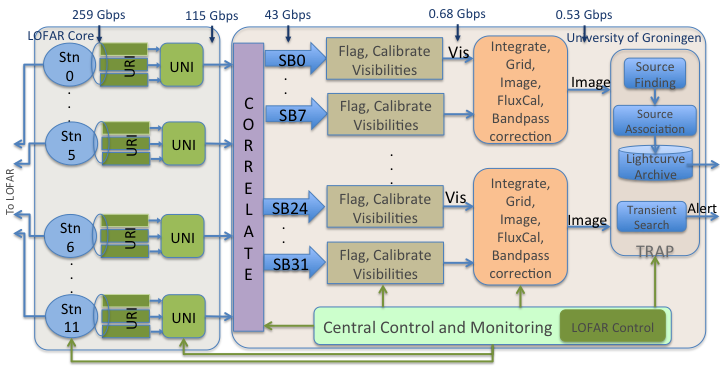
\includegraphics[width=1\textwidth]{Figs/Overall_arch_afaac/Slide1.png}
\caption {Overall  architecture of the  AARTFAAC all-sky monitor  depicting each
  processing sub block, along with the Monitoring and Control (MAC) system. }
\label{fig:afaac_arch}
\end{figure*}

The station  constitutes the first component  of the radio sky  monitor. This is
the only sub-system shared with LOFAR.  The AARTFAAC monitor consists of further
subsystems which are independent of  LOFAR processing.  Its overall architecture
is shown schematically in Fig. \ref{fig:afaac_arch}, and illustrates the main
processing  sub-blocks  of  the  instrument,  including  the  data  routing  and
processing blocks, as well as the control and monitoring flow.

The AARTFAAC  array consists of  12-stations from within  the core of  the LOFAR
telescope,  with inter-dipole  distances  ranging  from a  few  meters within  a
station, and a maximum of 1300m  (TODO) across stations. The exact core stations
of    LOFAR     constituting    the     AARTFAAC    array    are     shown    in
Fig. \ref{fig:afaac12_arrayconfig}.

\noindent  \textbf {Array  configuration:} The  choice  of the  subset of  LOFAR
stations used  in the AARTFAAC system  is dictated primarily by  imaging quality
and sensitivity, as well as due to constraints on the latency of calibration and
imaging. The central six stations of  the LOFAR telescope (called the superterp)
form a densely sampled UV plane, and are ideal for wide field imaging since they
are  co-planar to  high accuracy  (centimeter  level).  The  outer six  stations
provide higher sensitivity and resolution, and  have been chosen as a compromise
between the  UV coverage and the  extra processing due to  the W-component.  The
salient features of the LBA\_OUTER station configuration for the chosen stations
are     shown     in           Table     \ref{tab:afaac_specs}.      Figure
\ref{fig:afaac12_arrayconfig}  shows the  LOFAR stations  that are  part of  the
AARTFAAC system.

In contrast to  LOFAR, AARTFAAC processes the data of  each individual dipole in
order to achieve  all-sky imaging. Therefore a spigot for  each dipole signal is
created to  an independent processing architecture,  prior to the phasing  up of
dipoles within a LOFAR station.   This allows simultaneous observing with LOFAR,
leading  to high  availability of  the  AARTFAAC system.  Finally, the  AARTFAAC
system  has  been   built  on  top  of  LOFAR  primarily   due  to  the  extreme
configurability offered by LOFAR signal processing.  However, this restricts the
layout of  the antennas  within a  station as well  as the  stations themselves,
resulting  in   a  sub-optimal  configuration  from   the  transients  detection
perspective.  This results,  e.g., in  gaps in  the instantaneous  12-station UV
coverage,  and the  need  for  W-projection due  to  non-coplanarity across  the
stations.  Recognizing  this, the  co-planar AARTFAAC-6  array remains  a viable
sub-system for certain science cases.


To summarize  the AARTFAAC processing, a  user selected subset of  subbands from
every  dipole is  transferred  as  UDP packets  over  a  dedicated 10Gbit  fiber
connection  to  the  central  processing  systems.   These  are  received  by  a
streaming, real-time  software correlator  implementation which aligns  the data
and estimates the spatial covariance matrix  between every pair of dipoles.  The
generated visibilities  are streamed  over TCP/IP to  a calibration  and imaging
pipeline component  which carries out  autonomous imaging.  The images  are then
analyzed    by   a    software    tool   (The    Transients   Pipeline,    TraP,
\citep{swinbank2015lofar}), which  extracts the  light curves of  sources within
the image,  and analyses them for  variability using a number  of parameters.  A
(planned) trigger  generation subsystem  will publish  reliable triggers  in the
form  of VOEvents  \cite{williams2006voevent},  which can  be  claimed by  other
telescopes to observe candidates with high sensitivity and resolution.



\begin{wstable}[h]
\caption{Specifications of the AARTFAAC All-sky radio monitor.}
\begin{tabular}{@{}cccc@{}} \toprule
Parameter & Specification & Units & Comment\\ \colrule
Frequency range & 10-90 & MHz & Assuming LBA processing  \\
Processed bandwidth & 6.25 & MHz & Processing 32 subbands \\
Maximum baseline & 1000 & m & In LBA\_OUTER station array configuration\\
Resolution & 30 & arcmin & \\
Usable field of view & 130 & deg & SNR of TODO \\
Sensitivity & 14 & Jy & 8 Subbands gridded on a common grid \\
Frequency resolution & 1.56 & MHz & For transient detection. \\
 & & & Buffered visibilities at 3kHz resolution.\\
Time resolution & 1 & sec.\\ \colrule

\end{tabular}
%% \begin{tablenotes}
%% \item[a] Sample table notes.
%% \item[b] Sample table notes.
%% \end{tablenotes}
\label{tab:afaac_specs}
\end{wstable}

\begin{figure*}[htbp]
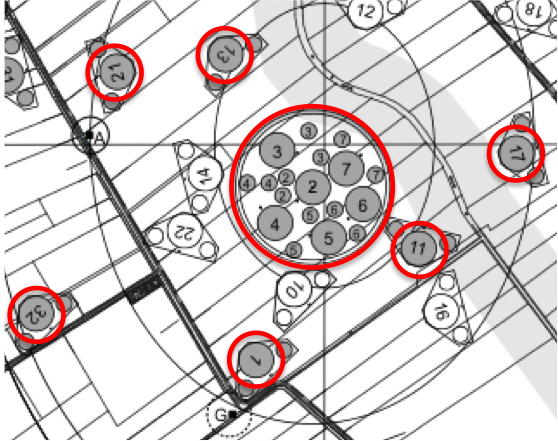
\includegraphics[width=0.5\textwidth]{Figs/afaac12_arrayconfig.png}
\caption{The spatial distribution of AARTFAAC-12 stations within the core of LOFAR stations.}
\label{fig:afaac12_arrayconfig}
\end{figure*}


We describe the various subsystems making up the AARTFAAC All-sky monitor in the
following sections.

\section {\label{sec:station_hardware} AARTFAAC Station Level Processing}
In  this section  the station  level instrumentation  relevant for  the AARTFAAC
system is discussed.  This involves systems which were already  present in LOFAR
stations, as well  as the additional instrumentation added  specifically for the
AARTFAAC system.
\subsection {Receivers}  The  antennas  in the  field  are connected  to
Receiver Units  (RCU). On those boards  the antenna signals are  amplified, band
pass limited  and converted into  the digital  domain.  The antenna  signals are
sampled with a 200 MHz clock frequency  delivering a bandwidth of 100 MHz to the
digital processing  system. The  A/D converter  uses a  sample resolution  of 12
bits.

\subsection  {LOFAR Digital  Processing}  The  LOFAR digital  processing
boards, also  referred as  Remote Station  Processing (RSP)  boards are  used to
channelize  the 100  MHz bandwidth  into  1024 subbands.  The channelization  is
implemented with a 1024-tap PolyPhase  filter bank implementation on each dipole
input. The output of  this filter bank is used for both  LOFAR and AARTFAAC. The
filter  bank analyzes  the sampled  voltage  timeseries into  a complex  voltage
spectrum  of 512  subbands. Thus,  the  entire analog  band of  the LBA  between
10-90MHz is available for further processing.

The output, for a set of 1024 real voltage samples, consists of a complex number
per  subband,  with a  2s  complement  16-bit  representation  of the  real  and
imaginary components.  A  single RSP board can handle the  processing of sampled
data from 4 dual polarized antennas. Since a LOFAR station is made up of 48 dual
polarized dipole antennas, 12 RSP boards are required per station. This is shown
in  Fig.  \ref{fig:afaac_station_hw}.   For  LOFAR, these  subbands are  further
processed in the RSP boards to  form spatially directed station beams by phasing
up the information from each antenna for  every subband. In order to combine the
information  of all  antenna signals  the RSP  boards are  connected via  a ring
network. For  LOFAR observations each  RSP board  is responsible to  calculate a
partial  beamformed  sum  of  the  antennas connected  to  that  particular  RSP
board.  It  further  adds  this  to the  result  received  from  its  preceding
neighbour, and  routes the partial sum  onto the ring network  to its succeeding
neighbour.  In  this  way the  last  board  in  the  ring calculates  the  final
beamformed sum, resulting in a spatially directed station beam.

The ring network consists  of four 2 Gbps links from one RSP  board to the other
by  daisy chaining  their  serial I/O  links.   These links  are  also used  for
AARTFAAC, since there was free capacity left over.  Therefore, it is now used to
carry LOFAR specific  data products (partial sums), along with  the raw AARTFAAC
subbands. Of  the total  8Gbps bandwidth of  the ring network,  about 6  Gbps is
occupied by LOFAR  specific products, with the remaining  bandwidth carrying per
dipole subbands used exclusively for AARTFAAC processing.
%% Station level  beamforming in  a particular  direction requires  calculating the
%% weighted sum of  all dipoles of the same polarization,  with the applied weights
%% being dependent on  the direction of beamforming.  Each  RSP board fundamentally
%% generates the  beamformed product for  its 4  client dipoles for  every subband.
%% These are termed  as 'beamlets'.  The necessary exchange of  beamlets with other
%% RSP boards to  create the station beam is achieved  via the interconnect between
%% the various RSP boards.\\

%% Each data  product from the RSP  signal processing is encapsulated  in a packet,
%% and marked with a datatype magic number. This allows differentiation between the
%% generated data products.

To enable the generation of the AARTFAAC data the RSP firmware on the FPGAs have
been modified. The AARTFAAC specific firmware  selects a subset of the available
512  subbands   of  all   antennas  specifically   and  independent   of  LOFAR.
Unfortunately, the available  ring network data bandwidth  forms the fundamental
limitation of the AARTFAAC processed bandwidth.  To retrieve more bandwidth, the
firmware accommodates  a configuration in the  number of bits used  to represent
the complex filtered output per subband.  Thus, bandwidth can be traded with bit
width, or the dynamic range in the filterbank outputs.  The bit mode of AARTFAAC
can be  set completely independently of  LOFAR's choice of bit  mode. The choice
between the various bit modes depends on the RFI environment of the observation.
An  8-bit complex  representation of  the filterbank  subbands are  found to  be
adequate for almost all observing conditions except during severe RFI.

The bandwidth available to AARTFAAC is limited to 36 subbands in 16-bit mode, 72
subbands in  8-bit mode, 108 subbands  in 5 bit  mode, or 144 subbands  in 4-bit
mode.  This allows  AARTFAAC to  achieve  high sensitivity  by placing  subbands
contiguously,  and later  integrating them,  while  at the  same time  achieving
spectral coverage  by placing subbands to  sample a larger extent  of the analog
spectrum. In the rest of the document, we refer to 8-bit subbands.\\

\noindent \textbf  {Sampling clock and  Timing:} This sub-system is  shared with
LOFAR.  A  clock  distributor  board  (SyncOptics) at  the  center  is  used  to
distribute  a 10MHz  reference  to every  one  of the  24  core LOFAR  stations,
including the 12  AARTFAAC stations.  The 10MHz reference is  generated by a GPS
disciplined  Rubidium  frequency  standard,  and   is  fed  into  a  Timing  and
Distribution Board  at the  station.  This board  generates the  200MHz sampling
clock required by the RCUs, and is also  used for the data processing at the RSP
boards. It  ensures that  an identical  (hence coherent) clock  is used  for the
sampling of data from the AARTFAAC stations.

The absolute time is communicated to the  RSP boards on station reset by the LCU
(local control  unit) as a 64-bit  timestamp counter. The RSP  board then embeds
this 64-bit timestamp  into the data packets  that it generates at  the start of
the next absolute second, indicated by a  PPS (pulse per second) signal from the
GPS timing  system.  Once set,  the station hardware  updates this counter  on a
derivative of  the available 200MHz  reference, thus ensuring that  the absolute
time  is  embedded  in  the  data  with a  resolution  of  a  single  sub-band's
time-sample ($\sim5\mu  sec$). The absolute timing  accuracy is of the  order of
the sampling clock period ($\sim5nsec$) due to the GPS 1PPS signal being sampled
on the ADC sampling clock.  All further aligning and timing of the incoming data
in  both LOFAR  and  AARTFAAC systems  is  carried out  based  on this  embedded
timestamp.

\subsection {AARTFAAC Piggy Back System}
The AARTFAAC  piggy back system  is implemented by URI  (UniBoard-RSP Interface)
boards. These  boards are installed in  the ring and basically  tap-off the data
from each ring interface. The ring data is  copied on the URI board. One copy is
forwarded to the next RSP board in the ring to guarantee the LOFAR observations,
while the other  copy is sent to  the AARTFAAC data router. Thus,  the URI board
ensures high availability via simultaneous operation of LOFAR and AARTFAAC.

Each URI board  interfaces with the serial  I/O links of 4 RSP  boards.  The URI
board  further implements  the first  stage of  the overall  transpose operation
required  to bring  coincident  data of  all  dipoles for  a  single subband  to
consecutive memory locations.  It does so  by statically routing upto 9 subbands
from all  dipoles available on the  4 RSP boards  to a single output  lane. Each
incoming link  contains 36  subbands from  8 dipoles,  while each  outgoing link
contains  9  subbands   from  32  dipoles.   This  operation  can   be  seen  in
Fig. \ref{fig:afaac_station_hw} in the data-flow  layout between the URI and the
UNB, which  shows the collation of  data from 9  subbands for 32 dipoles  onto a
single data  link.  Altogether, three  URI boards  are adequate to  transfer and
transpose 36 subbands at 16-bits into the Uniboard based router for all antennas
within a station.\\

\noindent  \textbf {AARTFAAC  Data Router:}  The  data router  is the  interface
between the station  level instrumentation and the next  signal processing unit,
the   correlator.    The   data   router  is   implemented   with   a   UniBoard
\citep{gunst2014application}.  The  board consists  of 4 upstream  FPGAs (called
back-nodes)  connected  to  the  URI  boards, and  4  downstream  FPGAs  (called
front-nodes) to connect to  the correlator over a long haul  fiber link. Each of
the back-node  FPGAs receives 9 consecutive  subbands out of the  36 subbands in
the URI board  output.  However, output bandwidth constraints  from the stations
to the central signal processing limit the back-nodes to transferring 8 of the 9
subbands onward.

A second level  of data rerouting is  carried out at this stage  such that links
from the 3 different URI boards (each containing 9 subbands from 32 dipoles) are
connected to the same back-node.  This  allows the back-node to collect the same
subbands from all 96  dipoles making up the station, into  a single output link.
These data are transported to a single Front-node FPGA.  The latter encapsulates
the  data into  a UDP  packet  which is  transmitted  on a  long haul  10Gigabit
Ethernet interface to the remote  correlator.  A single Uniboard interfaces with
two 10Gbps links to a switch which is connected with a single 10Gbps link to the
central processing machines,  located at the University of  Groningen about 50Km
away.  Each  link carries about  9.8Gbps of data,  consisting of 32  subbands of
8bits from all dipoles in the station.\\

%% \noindent  \textbf {Data  rates  and bandwidth  limitations:  } The  fundamental
%% limitation  to  AARTFAAC  processed  bandwidth is  presented  by  the  bandwidth
%% available  on  the ring  network,  and  depends  on  the bit-mode  chosen.   The
%% bandwidth available  to AARTFAAC is  limited to 36  subbands in 16-bit  mode, 72
%% subbands in  8-bit mode, 108 subbands  in 5 bit  mode, or 144 subbands  in 4-bit
%% mode.  A  random selection of  subbands from the  available 512 can  be inserted
%% into the  available AARTFAAC slots on  the ring network.  This  selection can be
%% made via  manipulation of the control  registers of the RSP  board.  This allows
%% AARTFAAC to achieve high sensitivity by placing subbands contiguously, and later
%% integrating them, while at the same  time achieving spectral coverage by placing
%% subbands to sample a larger extent of the analog spectrum.\\

%% The stations operate on a fixed sampling  clock of 200 MHz, leading to an output
%% rate of ~12  Mbps per dual polarised dipole antenna  per 16-bit complex subband.
%% The limited ring network bandwidth of a  station allows only 36 of the available
%% 512 subbands of 16-bits from all dipole antennas (total bandwidth ~20Gbps) to be
%% carried to  the URI board.  The  station Uniboard further restricts  the sampled
%% bandwidth to match its output bandwidth into 2x10Gbps links.  Of the incoming 36
%% subbands, only  16 are forwarded  for correlation.   Each 10Gbps link  carries 8
%% subbands, corresponding to ~4.5Gbps of data.

\noindent \textbf {Monitoring and Control  interface:} Every station is equipped
with a  Local Control  Unit (LCU), which  is a computer  system running  a Linux
operating system.  These systems are networked  to the LOFAR control system, and
also act as Network Time Protocol  (NTP) clients. Thus, their absolute times are
aligned to  better than a  few milliseconds. The  control of the  remote station
electronics consists of  two layers. Firstly, Command and  Status Registers have
been  opened up  at the  FPGA level,  and can  be accessed  via a  dedicated and
separate control  Gigabit Ethernet interface  to the hardware  boards. Secondly,
the  LCU provides  an  abstraction layer  between the  hardware  and the  global
control system  via a user accessible  tool and driver combination.  All control
and monitoring commands  from a global control system are  addressed to the LCU,
with the hardware driver ultimately  communicating the commands over the Gigabit
Ethernet control link to the RSP boards of the station.

% \begin{figure*}[htbp]
% \centering
% 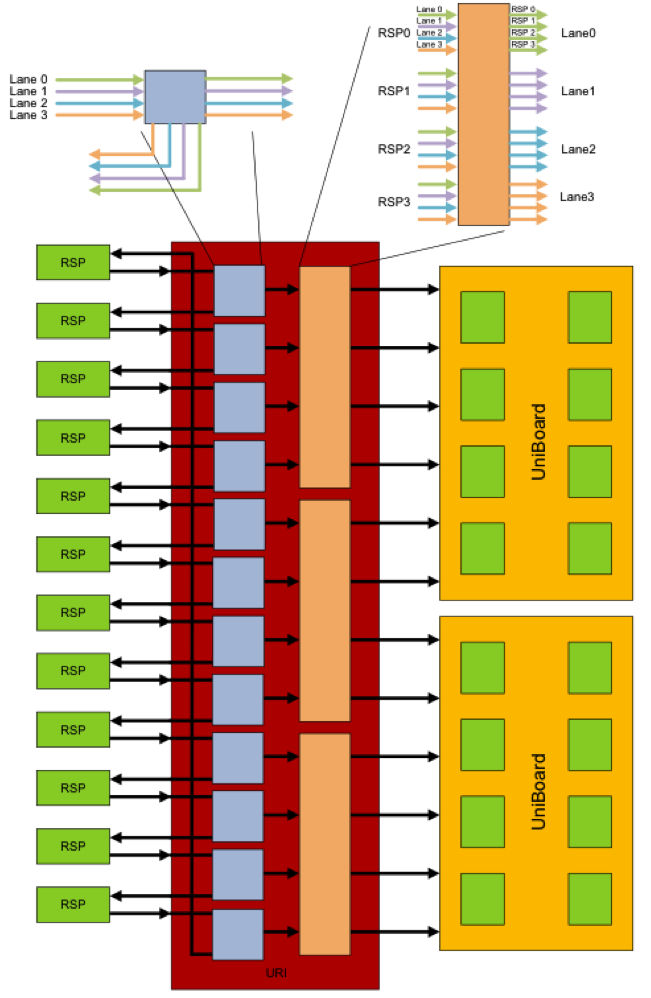
\includegraphics[width=0.75\textwidth]{Figs/station_hw_proc_afaac.png}
% \caption{The station level hardware changes  allowing creation of a coupled data
%   path for AARTFAAC data flow.}
% \label{fig:afaac_station_hw}
% \end{figure*}

% Figure \ref{fig:afaac_station_hw} depicts the  station level ring network, whose
% bandwidth is shared between the beamformed  subbands as well as the dipole level
% subbands. The ring network bandwidth constrains the processed AARTFAAC bandwidth
% to  a fundamental  maximum of  36 16-bit  subbands, or  about 7  MHz, while  the
% Uniboard  interface further  restricts the  bandwidth to  8 subbands  per 10Gpbs
% output link. The URI boards in combination  with the uniboards carry out a first
% level of the incoming data transposition.

\section {\label{sec:gpucorr} The AARTFAAC real-time correlator}
\begin{figure*}[htbp]
\centering
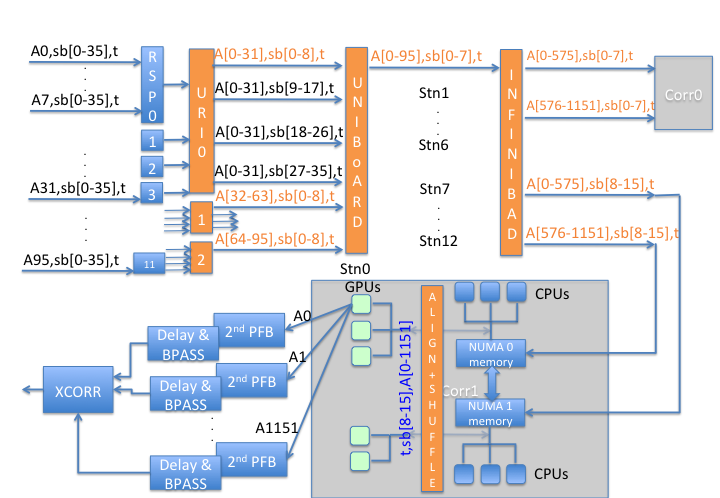
\includegraphics[width=1\textwidth]{Figs/data_routing_transform_hierarchy/Slide1.png}
% \caption{The GPU  correlator implementation  using a pair  of Xeon  class server
%  machines hosting AMD GPUs}
\caption{The hierarchical  data processing and routing  necessary for optimizing
  correlator  compute  performance   on  GPUs.  Here,  the   flowing  data  is
  represented by the triad of $[di,sb[i-j],t]$, where di refer to an individual
  dipole, sb[i-j] refer  to the range of  processed subbands, and t  refers to a
  time  sample.  The orange  blocks  correspond  to hierarchical  elements  that
  shuffle data }
\label{fig:afaac_station_hw}
\end{figure*}

The correlator  subsystem estimates the  spatial coherence between all  pairs of
dipoles in the system per frequency channel, and time integrates the signal down
to 1 second.  With 12 stations, each containing 48  dual-polarized antennas, the
total number  of dipoles  is 1152,  making the correlator  one with  the highest
number of spatially distinct input streams among contemporary instruments.  This
is the most computationally intensive subsystem  of the pipeline, and the entire
data routing  hierarchy is fashioned  to lay  out the data  such that it  can be
optimally operated on by our chosen compute architecture.

Its  input is  formed  of the  subbanded complex  voltage  timeseries from  each
polarization of  every antenna.  The output  consists of a timeseries  of dipole
array covariance matrices with a chosen time and frequency averaging.

The correlator ingests about 9.7 Gbps per station in real-time, corresponding to
32  subbands of  8bits for  each  of the  1152  dipoles.  It  needs to  produce
channelized data  from the subband  inputs due  to requirements of  flagging and
calibration. The resulting  computation is theoretically about  ~5 TFLOPs, to be
carried out  in real-time,  with minimum  latency.  A  major requirement  was to
minimize  development  effort,  which   effectively  eliminated  an  FPGA  based
approach.

Of the available  approaches, a heterogenous architecture  consisting of general
purpose  CPUs in  combination with  Graphical Processing  Units (GPUs)  has been
found to be the  best match between our requirements of  ease of development and
performance.  Compared  to contemporary  multi-core CPUs and  DSP architectures,
GPUs have  been found  to have  the best performance  and energy  efficiency for
algorithms  relevant  to  channelizing  and  correlating  radio  astronomy  data
\cite{romein2016comparison}.   The correlation  operation has  a low  Arithmetic
Intensity, implying that the data brought to  a device ALU is operated on only a
few times.  This, combined with  the relatively restricted I/O bandwidth between
the host CPU and the device GPU, has  been used as an argument against using GPU
systems for correlation.  However, with increasing number of signal sources, the
I/O  requirements   scale  linearly,   while  the  compute   requirements  scale
quadratically.   Thus, a  large enough  input  system can  make the  application
compute bound. This  is the case with  the AARTFAAC system.  The  latest GPUs on
server class machines come close to  meeting our requirements of dense computing
and high bandwidth I/O between CPUs and GPUs.

Our  correlator  implementation  shares  ancestry   with  the  LOFAR  GPU  based
correlator architecture,  which also  needs real-time  processing to  reduce the
large  volumes of  data being  produced.  However,  LOFAR deals  with far  fewer
station input streams due to station level beamforming.


%% The signal processing blocks necessary to achieve the correlator specs are shown
%% within the  GPU block  in Fig.  \ref{fig:afaac_station_hw}.  After  the incoming
%% subbanded  data from  each station  is collated  and time  aligned, a  Polyphase
%% filter bank is  implemented in order to increase the  frequency resolution.  The
%% resulting channels are then  compensated  for the fixed cable delays in the
%% system, as well as for the bandpass response of the first stage Polyphase filter
%% bank.  Following  this, signals from  corresponding timeslices for  all stations
%% are correlated. The generated covariance matrix  is then written out for further
%% processing.

\subsection  {Implementation  Hardware  architecture:} 
The heterogenous  The AARTFAAC  correlator is  made up  of server  class machine
utilizing multiple  GPU devices  tocarry out the  computation necessary  for the
correlation.  The  host CPU  based machines  acts as  the interface  between the
station data and the GPU devices.  They  implement the data reception and collation, and arbitrate
the data distribution between different GPUs. 

%% GPU h/w  architecture summary: Each  card has 2  GPUs with the  Graphics Core
%% Next(GCN) architecture,  and 2x6GB  device global  memory.  A  GPU has  28 CU
%% arrays, where  each array  has 4  CUs coupled tightly  together with  some L1
%% cache. Each CU consists  of a set of 4 SIMD  structures.  Each SIMD structure
%% consists of 16 ALUs,  cache and some addressing logic to  bring the data into
%% them.  A single  instruction is provided to each SIMD  structure, and this is
%% executed on  all 16 ALUs  (hence SIMD).   Since each CU  has 4 SIMDs,  it can
%% handle 4  instructions in parallel,  where each instruction is  being carried
%% out on a set of 16 datapoints.

%% Work-item : Is the  computation running on a single ALU of  16 within each of
%% the 4  SIMDs of  a CU. 64  work-items to  a CU.  Each of the  4 SIMDs  can be
%% working on a different wavefront.

%% Work-group: Is the set  of CUs making up 1 CU array  (=4 CUs). Coarse grained
%% parallism

%% Wavefront : Is a vector of data on which computation has to occur. The vector
%% size  is  a  multiple of  the  SIMD  ALU  size  (16). Size  is  typically  64
%% work-items.  Adv:  Single global addr.  space between host and  device memory
%% via on-board  virtual memory. On  board instruction scheduler to  avoid blank
%% slots in instr. execution.  fma has  higher accuracy and is faster than using
%% traditional single precision operations.



The  implementation  consists  of  two identical  machine  configurations,  each
capable  of processing  16  incoming  subbands from  12  stations. Each  machine
consists  of  dual Xeon-class  processors  with  24  cores  each. The  CPUs  are
connected to  32 GB  of memory each,  operating in a  Non Uniform  Memory Access
(NUMA)  configuration. Five  AMD  FirePro  S10000 GPU  cards  are available  per
machine,  interfaced  to  the  CPUs   over  8x16bit  PCIe  lanes  (TODO:  Verify
correctness). To receive the ~9.7Gbps data  output from each of the 12 stations,
both  servers are  equipped with  2x40Gbps Ethernet  interfaces, each  interface
receiving half  the bandwidth  of data  from 6 stations,  and also  carrying the
output correlations to downstream processors.\\

\noindent  \textbf  {High  bandwidth  switch:} An  intermediate  high  bandwidth
Ethernet switch (Mellanox ConnectX-3 MT27500),  in combination with the Uniboard
data router, is utilized to carry out the last stage transform of the per dipole
data stream. This  results in the same  subset of subbands from  all 12 stations
being transmitted to the same server, 6 to each of the Ethernet interfaces.  The
Back-node  FPGAs of  the Uniboards  encapsulate  data such  that a  subset of  8
subbands from 6 stations have an identical  destination IP address of one of the
interfaces. Thus, as shown in Fig. \ref{afaac_station_hw}, half the bandwidth of
the first  6 stations goes  to interface  0 of corr0,  the same subbands  of the
remaining 6  stations goes to  interface 1 of corr0.  The remaining half  of the
bandwidth goes in a similar fashion to the corr1 machine.\\

\noindent  \textbf  {NUMA  domains:}  A  NUMA CPU  and  memory  architecture  is
necessary in order  to receive the incoming high bandwidth  data and to transfer
them to  the GPUs,  as well as  to manage  the last stage  data exchange  of the
6-station  data   between  CPUs   controlling  the   two  Ethernet   cards  (see
Fig. \ref{afaac_station_hw}).  The  resources available to a  single machine are
organized into two NUMA domains on  that machine, with each domain handling data
from 6  stations. Each  domain includes  a 40Gbps Ethernet  interface, a  set of
processing cores, and the 32GB  memory associated with them.

However, the split of  the 5 GPU cards cannot be  made symmetrically between the
two domains, leaving one  domain with 3 GPUs, while the other  domain as 2 GPUs.
The  NUMA domains  allow  binding  of threads  handling  I/O  and processing  to
preferred  CPU  cores.   This  prevents thread  migration  across  cores,  which
increases data  locality in the core  caches.  Finally, thread binding  to cores
within a  NUMA domain allows routing  of network interrupts to  preferred cores.
This is essential for ensuring throughput of the system.

\subsection {Implementation of functional  blocks:} 

In this  section, we provide a  description of the implementation  of individual
functional blocks on our target hardware.\\

\noindent \textbf  {CPU Data collation and  time alignment:} The raw  data input
packets from individual  stations need to be collated for  an entire integration
period in host memory,  before being shipped to the GPUs  for correlation.  4 of
the  24  available processor  cores  in  a NUMA  domain  are  allocated for  the
execution of a  thread pool for the Ethernet I/O  handling.  Six Bounded threads
are created to run  on these 4 cores, one per input station.  The 6 station data
being received by the  alternate NUMA domain needs to be  collated into a single
buffer. This is carried out by  exchanging half the subbands for stations across
NUMA domains.   The incoming  subbands from  each station also  need to  be time
aligned before further processing.\\

Both effects are  achieved by setting up  a large, per subband  3-D buffer (with
axes of  time, station  and subband)  for the incoming  data. The  input threads
convert the  incoming data from signed  integer to float, and  placing them into
the correct time, station and subband slot  within the 3D buffer.  The number of
missing time slots  is also logged, and  is used to generate  a weighting matrix
for the  estimated integrated visibilities.   The aligned and  collated subbands
are  then  ready  to  be  transferred  to a  GPU's  global  memory  for  further
processing.

The  interface to  the openCL  runtime  environment is  via a  Queue onto  which
available GPUs in the same NUMA domain  line up for claiming data belonging to a
sub-band.  Once claimed,  the raw data is transferred asynchronously  to the GPU
device memory for  further processing. Each compute unit of  the GPU runs groups
of light-weight threads that cooperate on a single task, usually follow the same
instruction path,  share a piece of  fast local memory, and  synchronize through
barrier instructions.

Thus, a GPU thread group is serially  created for the execution of every logical
block.  The  blocks which operate at  the dipole level are  loosely coupled, and
suitable  for a  coarse-grained parallel  approach.  This  includes all  kernels
except the  correlation kernel.  Prior to executing  the correlator  kernel, the
data needs to be  transformed again in order to align the  data along the dipole
dimension. The transformed data is then passed to the correlator kernel.

The OpenCL  runtime environment  compiles the  GPU kernel  code in  runtime, and
produces the  assembly code to be  executed by the GPU's  Compute Units. Neither
the Texture memory, nor the render outputs  of the GPU architecture are used.

%% To  optimize performance,  the  work-unit splits  the data  such  that only  the
%% register file per CU is utilized at every stage.\\

\noindent  \textbf {Polyphase  Filterbank kernel:}  The first  signal processing
block  is  a  PolyPhase  filterbank,   applied  onto  the  single  subband,  and
constituted  of a  256-tap FIR  filter, followed  by a  1-D complex  FFT of  the
filter outputs.  The FFT is carried  out using an openCL  library, while the
FIR  filter  is implemented  to  maximize  the usage  of  the  GPU compute  unit
registers. The output is saved in the device global memory.\\

\noindent \textbf {Delay,  Bandpass Compensation and Transpose  kernel:} A delay
compensation is applied  to the channelized data to account  for the fixed cable
delays of  the dipoles with  respect to a  reference antenna.  These  delays are
obtained via a separate calibration, which is typically carried out at a cadence
of  a few  months.  The  delays  are available  in calibration  tables, and  the
frequency resolution  is high  enough to  apply them as  phase rotations  of the
visibilities.

The first stage polyphase filterbank implementation  in the RSP board results in
a deterministic  amplitude modulation  on the subband  bandpass, and  leading to
unequal powers in each subband channel.  This is demodulated via the application
of  a fixed  amplitude correction  by  applying channel  dependent weights.  The
resulting  data  is  brought  to   the  user  desired  frequency  resolution  by
integrating the channels.

Finally, the  fine-grained parallism axis  needs to be exchanged  from frequency
channels to dipoles, which requires a transpose of the data.

\begin{figure*}[htbp]
\centering
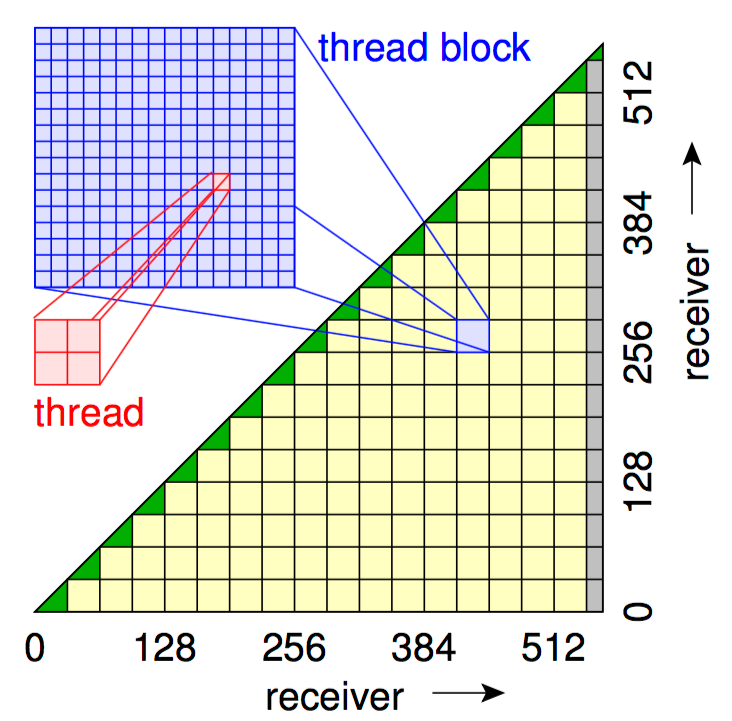
\includegraphics[width=0.4\textwidth]{Figs/ACM_spatial_split.png}
\caption {Depiction of the splitting of each output cell of a covariance matrix into triangles, rectangles and squares, which are computed by a compute unit of a GPU. From \cite{romein2016comparison}}
\label{fig:acm_spatial_split}
\end{figure*}

\noindent \textbf {Correlation kernel:}  Each dipole's subbanded and channelized
data is  then ready for correlation.   Depending on the user  input for specific
polarizations,  the   necessary  output   covariance  matrix   configuration  is
defined.  Only one  triangle  of the  hermitian covariance  matrix  needs to  be
computed. To distribute the computing of  the correlations among the GPU compute
units, the covariance  matrix is divided into squares,  triangles and rectangles
of outputs  to be computed,  as shown in Fig.   \ref{fig:acm_spatial_split}. For
our case, squares  of side 32x32 can  be assigned to a single  GPU compute unit,
and these  are further  split into  work-units of  2x2 covariances.  This choice
results in the best utilization of the compute unit register set for correlation
and accumulation, as well  as the use of a vectorized load of  4 floats into the
register set of the ALU.  The actual  correlation is carried out using the Fused
Multiply Add (FMA) instructions of the  GPU.  For single precision floats, these
can  be about  TODO\% faster  than non-fma  instructions.  The  post correlation
products are written  to device global memory by each  GPU execution thread.  An
event  is generated  on  the completion  of  the task,  and  the host  initiates
transfer of  the output  buffer to  host memory. The  timing and  weight related
meta-data is added to the correlations to form the record which is then streamed
out over a TCP connection to downstream processors.\\

\noindent  \textbf  {Asynchronous  host  to device  transfers  overlapping  with
  compute:} A source of throughput  bottleneck for the streaming, low Arithmetic
Intensity  correlator  application   on  a  GPU  platform   is  the  bandwidth
requirement for  the transfer of large  volume dipole data from  host to device,
and to a  smaller extent, the transfer of computed  correlations from the device
memory to the  host. The PCIe bandwidth limitation (TODO:  Is it just bandwidth,
or multiple access  to the same memory address?) can  be addressed by scheduling
data transfer asynchronously,  while overlapping the computation  of the kernels
with  the data  transfer.  This  has been  found to  have a  profound effect  on
throughput and latency.\\

\section {\label{sec:calim} Real-time calibration and imaging}
The real-time  flow of generated visibilities  need to be calibrated  and imaged
autonomously,  and  in bounded  time.   This  is  a departure  from  traditional
synthesis  imaging,  where the  long  observations  needed for  sensitivity  and
adequate UV coverage are bracketed  with observations of calibrator sources. The
over-sampled  instantaneous  UV  coverage,  the  wide  field  of  view  and  the
relatively poor  instantaneous sensitivity of  the AARTFAAC array results  in us
utilizing a model sky based multi-source self calibration approach, as described
in \cite  {prasad2014real}.  The  calibration and  imaging is  carried out  on a
cluster  of multicore  server class  machines, where each correlator output
subband is connected to a flagging and calibration pipeline see Figure
\ref{fig:afaac_arch}.\\

\noindent \textbf  {Autonomous flagging:} The realtime flagging scheme consists
of sigma clipping at two levels. Clipping is applied to the amplitudes of all
visibilities along the frequency axis and along the dipole axis. \\

\noindent \textbf  {Calibration and Imaging pipeline:}  The flagged
visibilities are amplitude  and phase calibrated  at the channel  level using a
simple point source model of  the four brightest sources (Cas.A, Cyg.A,  Vir.A,
Tau.A, termed the A-team) in the visible sky.  As  part of the calibration
process, the A-team sources are subtracted  out from the calibrated
visibilities in  order to reduce the  contribution  of  their  sidelobes   to
the  generated  images.\\  A  flux calibration is  then applied  based on  the
apparent fluxes  of the A-team during the  observation. The calibrated  per
channel visibility stream  of every subband is streamed out  again over TCP to
a machine  which implements the actual spectral and temporal integration to the
desired level.\\

Here, the channel outputs  of all subbands are ingested into  a large buffer and
ordered based on  their timestamps.  The spectral integration is  carried out by
gridding all visibilities onto a common  grid, while the temporal integration is
carried out by accumulation of the gridded visibilities. Prior to integration, a
quality control step based  on the rms thresholds on the  visibilities is run to
weed out  members of  the integration  set with  a high  variance due  to failed
calibration.  The Eigen3 \citep{eigenweb} C++ template library with its SIMD
support is  used to implement all stages of matrix processing and linear
algebra in general.  The calibrated and integrated visibilities are then
subjected  to tapering and weighting, before being Fourier  Transformed to
generate the final snapshot image.\\

\noindent \textbf {Buffered visibilities and images:} The final stage integrator
outputs a timeseries  of images per spectral integration unit.  These are passed
to the an image plane transient  detection pipeline (TraP), which can generate a
signal on the detection of a reliable candidate transient. Since the reliability
can be affected by the various operations like flagging, tapering etc.  that the
visibilities are subjected to, the integrator  has the ability to dump its large
internal buffer  of visibilities and images  to disk on receiving  a signal. The
dumped data can be then be processed more carefully.\\


%\begin {itemize}
% \item {Architecture, implementation choices, performance}
% \item  {Visibility  and  image  buffering strategy  for  followup  analysis  of
%   detected transients}
% \item {Quicklook images data path}
% \item {Unit test architecture}
% \item {Interface to TraP}
%\end {itemize}
\section {\label{sec:trap} Transient search methodology}
The  Transients  Pipeline  (TraP,  \citep{swinbank2015lofar})  carries  out  the
automated detection  of transients and  variable sources in AARTFAAC  images, in
near  real-time.  It  is  a  software package  optimized  for  the detection  of
transients in  radio images  while specifically dealing  with issues  related to
radio imaging, e.g., noise correlation or  PSF related issues.  It consists of a
collection of  python processes  carrying out image  processing, and  a database
which is  used to store  the image  processing outputs as  well as to  carry out
operations on the collective.  It operates  on a timeseries of image cubes (each
image cube consisting of two spatial and one spectral axis).

For any given image cube, it constructs  a catalog of all point sources (modeled
by elliptical Gaussians)  in every spectrally resolved image,  and compares them
against a database of point sources detected in previous timeslices.  The result
is the detection  of \textit{new} or \textit{variable} sources.   The former are
sources appearing  at locations where no  sources were seen in  previous epochs,
and the latter are sources which have been observed for multiple epochs and show
significant variability in their light curves. These results are computed on the
basis of the  multi-frequency light-curves for every detected  source, which are
available in the database.

The TraP  is the  real-time consumer of  the generated  multi-frequency AARTFAAC
images,  and produces  two  outputs: A  trigger  to the  outside  world in  near
real-time on  the reliable detection  of a short-duration transient  or variable
source,  and  a spectrally  resolved  database  of  lightcurves of  all  sources
detected in a timeseries of image cubes, together with time-resolved information
about their variability.  The latter is available for both real-time and offline
data mining, e.g., to implement different transient detection approaches.

Two aspects of TraP are interesting from the AARTFAAC perspective: The effect of
AARTFAAC  specific characteristics  on  the image  processing,  and the  overall
latency  induced by  TraP operating  in a  streaming mode.  We discuss  these in
greater detail below.\\

\noindent  \textbf  {Handling of  AARTFAAC  specific  characteristics by  TraP:}
AARTFAAC creates instantaneous, transit  mode (non-tracking) All-sky images, and
will be continuously monitoring the sky. The  very wide field of view results in
a varying sensitivity  across an instantaneous image, which has  to be accounted
for before  islands of  high SNR  pixels can be  decomposed into  sources.  TraP
approaches this by modeling the background (mean) pixel value and RMS across the
image by  estimating these values  within every cell of  a grid laid  across the
image, and interpolating the values over the full image.

In spite of resolutions of a tens of arcmin, sources in AARTFAAC images can have
significant positional  jitter due  to ionospheric  effects.  TraP  accounts for
these during its \textit{source association}  step, when it identifies whether a
detected source can be associated with an existing source in its database, based
on spatial  proximity.  Due to  the non-tracking  nature of the  instrument, the
AARTFAAC sensitivity pattern is fixed  with respect to local coordinates. Hence,
point sources  can have very different  SNRs when they traverse  the sensitivity
pattern as they rise and set.  They can  thus be classified as a new source when
their SNR crosses detection thresholds.  TraP accommodates such cases by keeping
track of  the fields-of-view and sensitivities  of all images it  processes, and
comparing a  detected source's  flux density  against recorded  sensitivities of
images  covering  the  same  area  to  check if  it  could  have  been  detected
previously.

TraP  calculates  two  variability  metrics  for every  detected  source  in  an
instantaneous image, and  per frequency bin $\nu$: the  flux density coefficient
of variation $V_{\nu}$,  and the reduced weighted $\chi^2$ as  a significance of
flux  density  variability, denoted  by  $\eta_{\nu}$.  Although they  are  time
aggregated values based  on the lightcurve of the source,  they can be generated
iteratively  via running  statistics,  and are  available  for every  timeslice.
Thus,  the streaming  nature  of  AARTFAAC images  can  be  accommodated in  the
existing framework.

Finally,  since  theoretically  the  AARTFAAC  image  stream  is  infinite,  the
lightcurve database  needs to  be truncated  in time.   Based on  the data-rates
generated  and current  computing capabilities,  a database  containing a  weeks
worth of lightcurves is manageable.  After  this, a new database will be created
for the next  weeks' observation. For requirements of  lightcurves with duration
longer than a week, wrapper scripts will be used to query the multiple databases
and construct required light curve.

Fig. \ref{fig:afaac_arch}  shows TraP as  the ultimate sink of  AARTFAAC images,
which will ingest 4 streams of image timeseries. Each stream corresponds to an 8
subband, 1second integrated image timeseries.\\

\noindent \textbf {Latency:}  TraP latency is contributed by  the source finder,
and the  database operation. The major  operations of the source  finder are the
RMS and background  map estimation, and fitting to detected  sources. The former
scales quadratically  with the number  of pixels  in an individual  image plane,
while the latter scales linearly with  the number of detected sources.  Database
operational times  have also  been shown  to scale linearly  with the  number of
sources detected  in an image. The  total compute times of  the sourcefinder and
the  database population  on AARTFAAC  data  have been  measured to  be under  a
second.


%% Ques  for Gijs:  -  Paper talks  about  storing  the image  cube  in memory.  He
%% mentioned a queue.  What is the effect  on latency?  - New  detections are first
%% checked to see whether  the region of sky where they are  seen has been surveyed
%% to  the   same  or  lower   sensitivity  where   the  source  would   have  been
%% visible. Supposing  there is a weak  source at low elevations  initially (so not
%% detected). When it reaches closer to the zenith, it will be detected, but should
%% not be classified as a new source, because


%%  - Variability detected  on timescales of seconds to years
%% - Cataloging process  is better  than an image  differencing approach  for radio
%% images. Also provides a light curve for  sources.  - TRAP was meant for RSM data
%% analysis, which  created a logarithmically  spaced timeseries of images.   - The
%% real-time mode  of Trap  will also  be used in  regular LOFAR  real-time imaging
%% observations.   - Trap  looks for  new  detections and  variability in  existing
%% sources. variability metrics  are retained on all sources.  -  Trap input is 3-D
%% image cubes, with a freq. axis.  - Output is near real-time alerts, and archival
%% database of lightcurves of all point sources, along with variability metrics.  -
%% src finding  and measurement process is  applied independently to each  plane of
%% the data cube, with point  sources parameterized by elliptical Gaussians. Source
%% association checks if the new measurements are updates on an existing source, or
%% a new detection.  -  Variability metrics are produced on a  per image basis, not
%% on a  complete timeseries. Variability metrics  can change with time  due to the
%% arrival of  new data.  -  Only stokes-I images  are searched for  transients.  -
%% AARTFAAC  will produce  extremely  large  number of  images,  this  needs to  be
%% factored in.  -  Every detected source has a running  catalog entry. All sources
%% in  an image  are first  attempted  to be  associated with  an existing  running
%% catalog entry.   - Since  a source  is deemed sacred  across the  frequency axis
%% (sources  found in  images at  different frequencies  at the  same location  are
%% associated with  the same  source in  the running  catalog) how  is the  case of
%% broadband images treated? When different parts  of the source can be brighter at
%% different freqencies?   - Null detections  (src was  expected, but not  found in
%% this  image)  lead  to forced  fits  at  the  catalog  position, with  the  peak
%% constrained to the  measurement at the catalog position.   - Variability metrics
%% are  updated for  every image  cube  that is  processed,  and a  history of  the
%% variability can be pulled from the database  in order to see how the variability
%% of sources evolves due to the addition of image timeslices.

\section {\label{sec:acontrol} The AARTFAAC Control System}
\begin{figure*}[htbp]
\centering
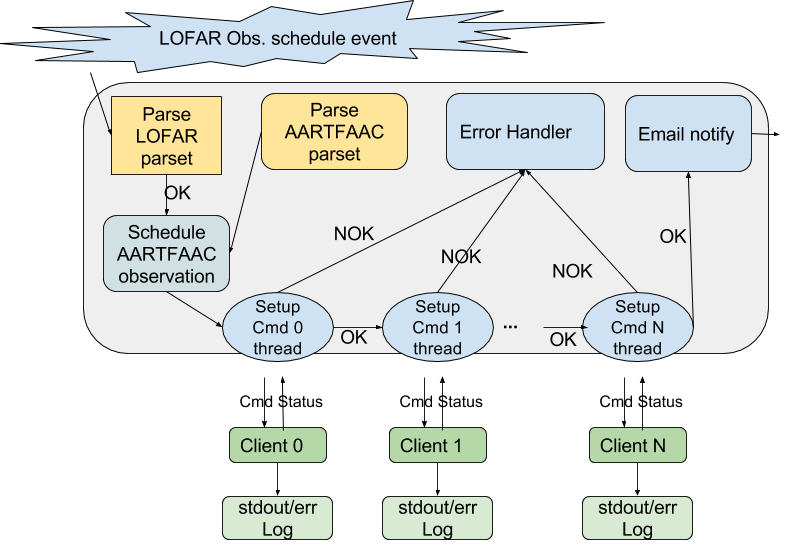
\includegraphics[width=0.50\textwidth]{Figs/afaac_ctrl_system.png}
\caption{The  control  system  architecture  which  interfaces  with  the  LOFAR
  observation scheduling system and triggers AARTFAAC observations.}
\label{fig:afaac_ctrl_sys}
\end{figure*}
The  AARTFAAC  control subsystem  coordinates  the  diverse processing  and
I/O infrastructure of the  AARTFAAC system, and acts as a  liaison between the
LOFAR observatory,  AARTFAAC user  and  system.   It is  essential  to the
autonomous functioning of  the instrument by  providing fault  tolerance.  It
has  a python based client-server architecture, with the  server process
existing on the LOFAR manager node and clients waiting for  commands on the
various AARTFAAC subsystem controllers. Every scheduled  LOFAR observation is
monitored  for suitability as an AARTFAAC  observation. Figure
\ref{fig:afaac_ctrl_sys} shows  the functional blocks of  the AARTFAAC control
system.   When a LOFAR observation is  initiated and AARTFAAC is allowed to
piggyback, the control  system launches  the  call-graph using  the  current
active  AARTFAAC configuration.  This  user defined configuration determines
i.e. what subbands to  listen to and how many  images to  create.  The
call-graph initiates  everything at  1 (stations, aartfaac tv,  pipelines) by
connecting to the appropreate clients and starting the processes. When at least
$1$ out of $n$ pipelines is started  and the stations are functioning properly
it calls everything at  $2$ (correlators and squashers). When at least $1$ out
of $n$ correlators and $1$ out of $n$ squashers have been spawned it will
initiate TraP in the third stage. An  email will be sent when an error occurs
or when an observation successfully started.\\

\noindent \textbf  {Monitoring interface:} The control  system allows
monitoring the  various  subsystems at  fine  granularity,  making  it useful
to  localize problems within  the system by examing the email reports.  For
monitoring dataflow on a hardware level we use
Munin\footnote{http://munin-monitoring.org}. This tool allows viewing
statistics  of I/O between nodes,  computing on various nodes,  and disk usage
via    a   webpage\footnote{https://proxy.lofar.eu/aartfaac/munin},
including history  at various time  cadences.  The processed outputs  at
various stages in the pipeline are also presented onto a
webpage\footnote{https://proxy.lofar.eu/aartfaac/index.html} for the end to
end, and astronomical monitoring  of the system, some  examples of this are
shown in the results section.

\section {\label{sec:results} Commissioning results}
\begin{figure*}[htbp]
 \begin {minipage}{\textwidth}
 %% \subfloat
   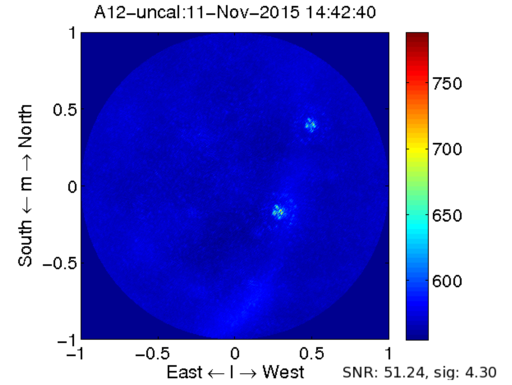
\includegraphics[width=\textwidth]{Figs/A12_uncal.png}
 %% \subfloat 
 %%  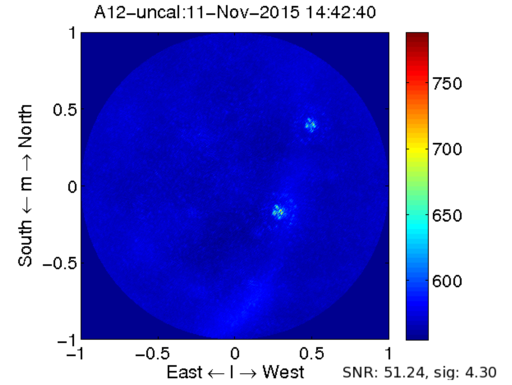
\includegraphics[width=0.3\textwidth]{Figs/A12_uncal.png}
\caption{An uncalibrated image from the 12-station AARTFAAC system, demonstrating the hardware data routing and  correlator functioning.}
\label{fig:afaac_results}
 \end {minipage}
 
\begin {minipage}{\textwidth}
 %% \subfloat
   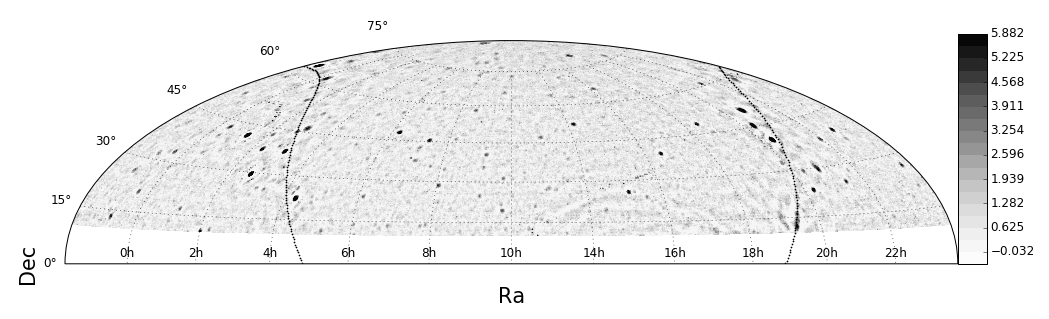
\includegraphics[width=\textwidth]{Figs/24hr_skymap_grey.png}
 %% \subfloat 
 %%  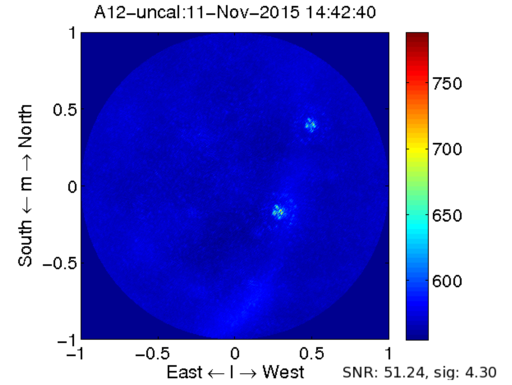
\includegraphics[width=0.3\textwidth]{Figs/A12_uncal.png}
\caption{A calibrated sky-map created from a 24hr observation from AARTFAAC.}
\label{fig:afaac_24hr}
 \end {minipage}
  
\end{figure*}
The AARTFAAC system is currently in place and operating with 6 LOFAR stations, a
total bandwidth of  ~3MHz, with real-time images being created  at a 1sec/192kHz
cadence. The correlator has been tested  to operate at the full specification of
12  stations  and  ~6MHz  bandwidth.  Fig.   \ref{fig:afaac_results}  shows  the
resulting All-sky snapshot image from the AARTFAAC monitoring webpage interface.

% \begin {itemize}
% \item {Overall latency of the system}
% \item {Long term performance of the entire system based on logs.}
% \item {Performance  in various  bit-modes, with  different number  of subbands,
%   expected sensitivity.}
% \item {Imaging quality Vs. latency: 6 station to 12 station.}
%\end {itemize}

\section {\label{sec:discussion} Discussion}
\begin{wstable}[h]
\caption{Overall latency budget and performance of AARTFAAC subsystems.}
\begin{tabular}{@{}cccc@{}} \toprule
%% & A-12 & A-6 \\ \colrule
Parameter & Compute time (ms) & Processing (TFLOPs) & Comment \\ \colrule
CPU data transform & 16.7 & 0.1626  \\
GPU FIR & 8.4 & 1.726\\
GPU FFT & 10.0 & 0.678  \\
% GPU Delay and Bandpass correction & 2441.0 & 0.0\tnote{a}  \\
GPU correlation & 212.9 & 4.824  \\
Online flagging & 74.3 &  & Thresholding visibility amplitudes across time and frequency\\
Calibration & 249 & & Both XX and YY pols, calibrating 63 channels.\\
 \colrule
Total & 571 & & \textbf{Measured latency on production systems} \\
 & & & \textbf {(upto calibration): 1100ms} \\ \colrule

Imaging & 40 & TODO & Gridding and FFT for 1 Stokes-I image per subband.\\ 
TraP & 696 & TODO & Measured with 4 input subbands on non-production desktop.\\ \colrule
\end{tabular}
\label{tab:afaac_latency}
\end{wstable}

%% \noindent \textbf {Signal Processing requirements:}
%% A variety  of signal processing  algorithms are  utilized in the  generation and
%% analysis of  real-time images from  AARTFAAC.  Here,  we describe only  the ones
%% relevant to  the real-time performance  of the  system, i.e., not  including the
%% characterization   of  transients,   and   only   discuss  their   computational
%% requirements.  Their  implementation and  performance  can  vary based  on  data
%% dimensions and its match to a particular computing architecture.

%% The first signal processing block is the Polyphase Filterbank, which essentially
%% consists of  an FIR  filter followed by  an FFT. This  filter splits  the signal
%% spectrally with a  lower scalloping and spectral aliasing loss.  The filter bank
%% can  be  represented by  TODO  Muls  and TODO  accs,  leading  to a  theoretical
%% requirement of TODO FLOPs for N. The FFT has a compute load of TODO FLOPs.

%% The subbanded signal is usually further filtered to a higher spectral resolution
%% by  a second  stage  filterbank. The  delay and  bandpass  correction involve  a
%% complex multiplication of  the signal with a static weight  vector, leading to a
%% load  of  TODO FLOPs  per  subband  for  TODO  output spectral  resolution.  The
%% correlation  is  carried  out  at   the  output  spectral  resolution.  For  our
%% specifications, this leads to a load of TODO FLOPs per channel per timeslice.

%% The Calibration  is the only data  dependent, iterative operation to  be carried
%% out in the  real-time chain. It consists of mainly  TODO matrix operations, each
%% costing  TODO.  The  total  expected  cost of  calibration  is  TODO  FLOPs  per
%% covariance matrix, assuming an average of TODO major and TODO minor cycles.

%% The Imaging consists of a weighting  operation on all visibilities, per spectral
%% unit. This  corresponds to a  cost of  TODO FLOPs/channel/sec. The  weighting is
%% followed by a gridding of the calibrated  visibilities onto a grid whose size is
%% dependent on  the image resolution  and field of view,  and with a  kernel whose
%% size is  also dependent on output  resolution. For our TODO  typical parameters,
%% this translates to  a cost of TODO  FLOPs. The generated images need  to be flux
%% calibrated, which  corresponds to  an element by  element multiplication  with a
%% correction matrix. This cost is about TODO FLOPs.

%% Once  the calibrated  images are  available, they  are passed  through a  source
%% finding stage, where islands of emission  are isolated into (point) sources, and
%% their properties ascertained by fitting 2D Gaussians to the emission island. The
%% source parameters are then recorded into a database for every timeslice, and the
%% timeseries is further analyzed for variability and for detecting transients.

%% \noindent \textbf  {Parallelization axis:}  Parallelization to handle  the compute
%% requirements can be carried out along  the temporal, spectral or spatial axis of
%% the incoming  data.  Organizing timeslices  for parallel processing can  lead to
%% latencies, which is inconsistent with the real-time requirement of AARTFAAC. The
%% spatially  distributed dipoles  result  in each  dipole  stream being  initially
%% processed  independently of  each other.   The correlation  process retains  the
%% spatial independence  since the generated  covariance matrix can be  split along
%% dipoles.   However,  the  processing  requires  alignment  along  the  time  and
%% frequency axis,  and further analysis  (imaging) fuses the spatial  axis.  Thus,
%% the  frequency axis  is  the  only truly  independent  axis  along the  complete
%% processing chain, with each subband or channel being processed independently.

%% Parallelization at different levels in the hierarchy is matched to the available
%% hardware architecture.  At upstream levels, the FPGAs operate in lock-step, with
%% no dynamic scheduling of data to processing units. An important task here is the
%% reorganizing of data along the frequency  axis such that the architecture of the
%% computationally intense components (correlation) can  be fully utilized. The CPU
%% offers   both  SIMD   via   vectored  instructions,   and   MIMD  via   multiple
%% cores.\footnote  {Flynn's  taxonomy:  SIMD=Single  Instruction,  Multiple  Data,
%%   MIMD=Multiple  Instruction,  Multiple Data}  [TODO:  What  is MIMD  used  here
%%   for?]. The  GPU offers  operations on  loosely coupled  data via  its multiple
%% compute units,

%% Since the data  from all dipoles is time and  frequency aligned when correlation
%% occurs,  parallelization  is fundamentally  on  the  frequency axis,  with  each
%% subband being processed  independently.  Within a subband, each  station data is
%% processed  independently till  the  correlation stage,  where a  synchronization
%% barrier is applied  to time align all  the dipole streams.  Each  channel of the
%% subband  correlation matrix  is also  processed independently  via a  GPU thread
%% group.  Further, a single channel covariance  matrix is broken into cells, which
%% are also computed independently.\\


\noindent \textbf {System performance:} The overall performance of the real-time
system  is quantified  by  the achieved  latency. Table  \ref{tab:afaac_latency}
presents  the  measured  compute  time  for various  functional  blocks  of  the
system. These  results have been  obtained for  the 6-station system,  since the
calibration  and  imaging  component  of  the 12-station  system  has  not  been
commissioned yet.  Thus, extrapolations on  the computation have  been generated
for the 12-station  system. All reported times have been  measured on production
systems, except for the TraP.

Here,  we  see  that  the  most   compute  intensive  functional  block  is  the
calibration,  whose compute  footprint  is dominated  by  the Weighted  Subspace
Fitting model source position determination sub-block. Alternative approaches to
this algorithm implementation will be  explored to reduce this cost. Calibration
latency can also  vary based on the observing conditions  like RFI occupancy and
the  presence of  the flaring  Sun. We  set an  upper limit  to the  calibration
iterations, trading off instrumental sensitivity to maintain latency.

The next  compute intensive component is  the correlator itself. Its  latency is
independent of missing  or poor quality data, since the  collated data buffer is
processed based on wall-clock time. Thread binding to CPU cores prevents process
migration,  and  the absence  of  competing  processes reduce  operating  system
induced non-deterministic latencies.

For the 6-station system, we measure a latency of ~1.1second to calibrated image
generation, on production hardware. This is about twice as expected from timings
of the compute  blocks. The remaining latency occupancy includes  times taken by
all compute blocks, as well as network and memory operation latencies. We expect
this  to  grow  by factors  of  2-3  in  anticipation  of the  more  complicated
calibration and imaging scheme for the 12-station AARTFAAC.

A streaming variant  of the TraP is still being  commissioned. Current profiling
reveals that  the source finding step  takes ~30\% of user  time, while database
operations to update the light curves  of detected sources take about 15\%. Both
these operations scale linearly with the number of detected sources in an image,
and thus  latencies on the  12-station images are  expected to be  only slightly
more.

\noindent  \textbf   {AARTFAAC  Scalability:}   The  AARTFAAC   All-Sky  monitor
implementation  can be  scaled  up  along the  spatial  (number  of dipoles)  or
spectral (processed subbands) dimensions. A  spectral scaling will ultimately be
limited by the ring network bandwidth to  about 64 subbands (~12 MHz) of 8-bits,
doubling the current  bandwidth. A spare 10Gbps link on  the uniboards can bring
the extra  32 subbands to the  center, where they  can be processed by  an exact
duplicate of the  current correlator system.  The choice of  a hierarchical data
transpose results  in the most efficient  final layout for correlation.   In the
generic  case,  following   the  same  design,  additional   subbands  could  be
accommodated by  increasing the levels  in the network hierarchy  to accommodate
the transpose.  The final correlation would  then be possible for the additional
subbands by replication of the frequency multiplexed hybrid correlator.

Keeping the  current bandwidth while increasing  the number of input  dipoles is
also feasible. The current Ethernet interface  allows another two stations to be
added.   The compute  requirements would  be almost  30\% higher,  due to  their
quadratic growth  with number of  input streams.  The correlation  operation has
been tested on the current GPUs for Scalability of the input streams, and should
be  able to  cope  with the  requirements of  the  extra inputs.   Accommodating
stations in addition to  the two mentioned here would likely  require data to be
transferred  between  multiple  CPUs  over  the  GigE  network,  which  will  be
prohibitively slow.\\

%% \noindent  \textbf {Impact  of sharing  dipoles with  LOFAR on  AARTFAAC:} LOFAR
%% operates using  either the LBA  or the  HBA antenna at  a time. Further,  due to
%% limited station level electronics for stations within the core, only a subset of
%% the available  station dipoles can be  utilized. This implies that  the AARTFAAC
%% telescope  is  dependent  on  LOFAR  for  the  choice  of  antenna  and  station
%% configuration,  reducing the  availability  for all-sky  monitoring. Within  the
%% station, only the LBA\_OUTER station  configuration is currently deemed suitable
%% for  real-time imaging.   This mode  of  LOFAR operation  favorable to  AARTFAAC
%% depends on  the observing  schedule and the  proposed observations.   Table TODO
%% shows some  statistics from previous cycles  on the fraction of  observing modes
%% favorable to AARTFAAC. Based on this, it may be reasonable to expect AARTFAAC to
%% operate TODO fraction of time, typically.\\

\noindent \textbf {Hierarchical  shuffling and transpose of  incoming data:} The
voltages  are available  as a  sampled  timeseries per  polarization, with  time
samples laid out contiguously in memory.  For efficient computing, these need to
be transposed such that the same  timeslice from all dipoles lie contiguously in
memory. This  operation involves transposing a  matrix of data with  a size NxN,
with N  being the  number of data  sources.  This memory  becomes inflated  by a
factor corresponding to  the number of time-samples in the  integration unit, as
well as the number of polarizations  being processed. Since the memory footprint
can be quite  large, this is quite  an inefficient operation due  to memory read
latencies etc.\\

We  achieve this  by spreading  the transpose  operation over  the nodes  on our
network. This is done in the following  manner: The URI boards carry out a first
level  of transposition  by physically  routing  a subbands  from a  group of  4
dipoles to a  single output.  The second  stage transpose is carried  out by the
Uniboard.  This  is at the  station level, and routes  all dipole data  from one
station as a contiguously laid  out group.  Finally, the inter-station transpose
to reorder data and  exchange the time axis for the station  axis is carried out
by the  CPU host component  of the  correlator. Here, the  PC memory is  used to
rearrange the incoming data and to carry out the transform. The resulting output
is then optimally laid out for correlation over all dipoles of the AARTFAAC, for
every polarization, and over the chosen integration time range.

%\subsection {Dynamic range and precision of computing}
%The 12-bit sampling (TODO: Confirm) provides  for a dynamic range of TODO. These
%raw data samples  are fed into the  hardware first stage PFB,  which carries out
%internal computation  on TODO bit  integer data,  and generates 16-bit  or 8-bit
%complex components (TODO: Is there any normalization at this stage? Why else are
%the actual numbers  so high?). Due to each dipole  sampled output being directly
%operated on without  any beamforming, the 8-bit dynamic range  has been found to
%be adequate for the AARTFAAC application.  Once the data reaches the correlator,
%all computations are carried out with single precision floating points.

\section {\label{sec:conclusion} Conclusions}
We  describe the  AARTFAAC All-sky  radio transient  monitor, an  autonomous and
real-time image  domain transient detection  machine piggy-backing on  the LOFAR
radio telescope. The  system consists of a diversity  of heterogeneous subsystems
ranging  from  FPGA  firmware,  to   heterogeneous  GPU  machines,  with  final
processing carried out on commodity computing  machines.  Its aim is to generate
real-time  triggers on  the detection  of reliable  transients, to  enable their
multi-wavelength followup.

Our implementation utilizes  a hierarchical routing of high bandwidth  data to a
central  correlator,  with co-processing  within  the  hierarchy to  spread  the
computing cost.  The most intensive computing  of the correlations of 1152 input
streams requires $\sim$  TODO TFLOPs, and has been achieved on  a system consisting
of 10 state-of-the-art GPUs.  Our system  operates in real-time, with an average
latency of TODO  seconds to the imaging, while generating  images with a dynamic
range of close to 2000:1 with a time and spectral integration of 1sec/190kHz.\\

%% The Scalability of  this system demonstrates the viability of  handling an SKA-1
%% like  sea-of-antennas approach  to enable  wide field  radio monitoring  at high
%% sensitivity.\\

\noindent  \textbf{Acknowledgments} This  work  is funded  by  the ERC  Advanced
Investigator  grant no.  247295 awarded  to Prof.   Ralph Wijers,  University of
Amsterdam.  We thank The Netherlands Foundation for Radio Astronomy (ASTRON) for
support provided in carrying out the commissioning observations.

\bibliographystyle{ws-jai}
\bibliography{ref}

\end{document} 
